\section{Debloating Results}
\label{sec:debloatingresults}

In this section, we begin by reporting statistics about our clustering. 
Next, we measure the performance of our debloating scheme and demonstrate its ability in reducing the attack surface of web applications. 
We report the performance of \sys{} and compare it to our baseline model through source code metrics such as LLOC reduction, as well as security metrics, namely CVE, gadget chain and CAC reductions. 
% Historically, research papers demonstrated the attack surface reduction of debloating schemes via the reduction in size of debloated applications.
% Other studies report the removal of historic CVEs and gadget chains as a means to measure the security gains of debloated applications. 
% We extend the existing metrics by measuring and reporting the number of calls to critical API.

\subsection{Clustering Statistics}
During our data collection step, we collected the code-coverage data from web application usage from 20 experts for each web application.
We then clustered their code-coverage information into 1-20 clusters. 
On one end, the code coverage information from all users are aggregated in a single cluster. 
On the other end, all users have their own uniquely debloated web applications that contains only the code that they have interacted with before. 
While \sys{} is capable of providing uniquely debloated web applications for each user, it is beneficial to keep the number of clusters low in order to reduce the complexity of separately maintaining $N$ applications. 

\subsubsection{Characterizations of \sys{} clustering}
For \sys{} debloating clusters, we look at statistics such as number of users in each cluster, as well as the high level roles of each cluster. 

For the web applications in our dataset, we observe a common list of tasks that are shared among the majority of users. 
For phpMyAdmin, virtually all users created new database and tables, executed SQL queries, and used the functionality of exporting and importing the database.
Some users also renamed or modified existing databases, dropped tables, or deleted rows of data. 
For WordPress, setting up themes and installing custom plugins, and creating new blog posts were among the commonly used features. 
Finally for Magento, creating new products, managing product inventory, and modifying prices were the most popular features. 

\begin{figure}[t]
    \centering
    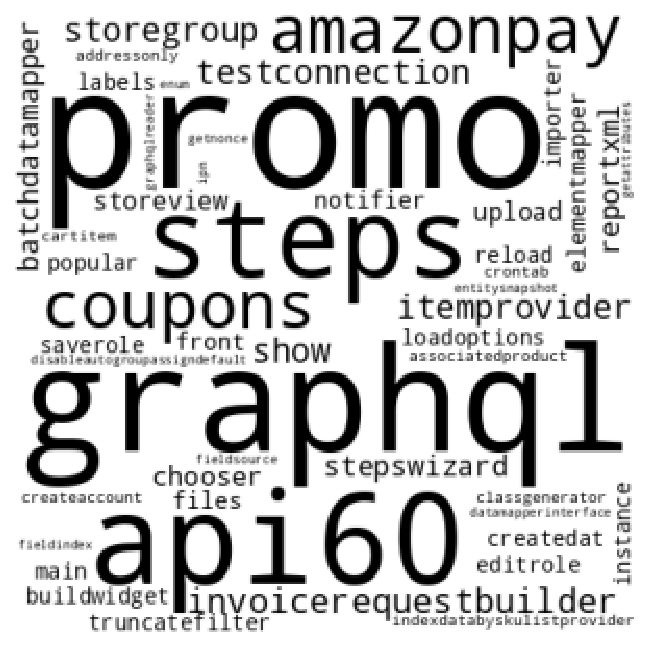
\includegraphics[width=0.5\textwidth]{figures/dbltr/magento_wordcloud.pdf}
    \caption{Word cloud of important terms for Magento cluster number four}
    \label{fig:magento_wordcloud}
\end{figure}

On the other hand, we observe patterns of feature usage that are unique to a subset of users. 
Among these user-specific features we observe exporting files with specific file extensions (e.g., CSV), using filters while displaying the query results, and modifying privileges. 
Similarly, Import/Export, modifying settings such as permalinks, RSS, and WXR are unique to certain clusters among the WordPress users. 
Finally for Magento, sales promotions, gifts and shopping cart rules, front end content modification, and sales analytics are among the unique features. 

We incorporate this observation into our clustering via the max-document-frequency parameter in TF-IDF. 
This way, we can ignore the common features that are used across all clusters and focus on the unique features when building the clusters. 

At this step, by looking at the most important terms for each cluster, we can assign a role title to the users of the cluster. 
Figure~\ref{fig:magento_wordcloud} depicts the word cloud of important terms for a sample cluster of administrators in Magento. 
Larger font size indicates a higher impact factor based on TF-IDF metric. In general, by analyzing the output of TF-IDF, we can define the following roles for clusters:

\begin{itemize}
    \item Mass actions (Delete, Copy, Refresh).
    \item Invoice, PDF, and Less files.
    \item Payment methods, Gift cards, and Refunds.
    \item APIs (GraphQL, XML), Promo, Coupons.
    \item Index, Cache, Internationalization (i18n).
    \item Cart, Suggestions, Recommendations.
    \item Guest purchases, Compare products, Shipping.
\end{itemize}

\subsection{Debloating results}
%By definition, debloating reduces the effective size of web applications. 
%In this section, we discuss the results of LLOC (Logical Lines of Code), CVE, and CAC (Critical API Call) reduction.

\subsubsection{LLOC Reduction}
 
We measure the reduction in size of web applications in terms of logical lines of code (LLOC), which counts the number of statements in the application source code. 
By reporting the size of the debloated applications in LLOC, we reduce the effects of various syntax and coding styles (i.e., the debloating process changing the code style after rewriting). 

Table~\ref{tab:lloc_reduction} shows the LLOC reduction results of our debloating scheme. 
The numbers are reported in terms of thousands of LLOC. 
The column marked as ``Baseline'' lists the debloating results of combining the code coverage data of all users together, which is equivalent to prior debloating approaches, such as the one by ``Less is More'' of Amin Azad et al.~\cite{lessismore}.
``\sys{}'' shows the LLOC statistics for the optimal number of clusters chosen by \sys{} for each web application, as determined by the Silhouette score described in Section~\ref{sec:num-clusters}. 
For \sys{} column, we report the size of the smallest (Min) and the largest cluster size (Max) along with the median. 
The number in the parenthesis for Baseline and \sys{} denotes the percentage of LLOC reduction with respect to the size of the original application. 

\begin{table}[]
    \caption{LLOC reduction of debloated clusters: Numbers are reported in terms of thousands of LLOC. For Baseline, and \sys{}, we report the percentage of LLOC reduction compared to the Original application.}
    \centering
    \scalebox{0.87}{
        \begin{tabular}{|l|l|l|lll|}
            \hline
            \multirow{2}{*}{\textbf{\begin{tabular}[c]{@{}l@{}}Web\\ Application\end{tabular}}} & \multirow{2}{*}{\textbf{Original}} & \multirow{2}{*}{\textbf{Baseline}} & \multicolumn{3}{c|}{\textbf{DBLTR}}                                                  \\ \cline{4-6} 
                                                                                    &                                    &                                    & \multicolumn{1}{l|}{\textbf{Min}} & \multicolumn{1}{l|}{\textbf{Median}} & \textbf{Max} \\ \hline
                phpMyAdmin                                                                          & 155                                & 44 (71\%)                          & \multicolumn{1}{l|}{31 (79\%)}    & \multicolumn{1}{l|}{39 (74\%)}     & 42 (72\%)     \\ \hline
                WordPress                                                                           & 103                                & 66 (36\%)                          & \multicolumn{1}{l|}{48 (53\%)}    & \multicolumn{1}{l|}{59 (42\%)}    & 65 (37\%)     \\ \hline
                Magento                                                                             & 1,050                              & 330 (68\%)                         & \multicolumn{1}{l|}{240 (77\%)}   & \multicolumn{1}{l|}{285 (73\%)}   & 318 (70\%)   \\ \hline
        \end{tabular}
    }
    \label{tab:lloc_reduction}
\end{table}

By comparing the LLOC reduction of Baseline to \sys{}, it becomes evident that a one-size-fits-all debloating (i.e., Baseline), exposes certain users and roles to a much larger code-base than they actually require. 
This unnecessary bloat for Baseline debloating can be as high as 30\% of extra LLOC. 
This unnecessary exposure is most significant for larger web applications such as Magento where certain users inherit up to 90,000 unnecessary LLOC which is 37\% larger---compared to the smallest \sys{} cluster---than what they actually need. 
Moreover, we observe that \emph{all} \sys{} clusters (including the one with maximum LLOCs) are strictly smaller than the Baseline approach, meaning that the globally debloated web application is still bloated as far as individual users are concerned.

\subsubsection{CVE Reduction}

One of the metrics to model the effects of debloating on the security of applications is removal of actual vulnerabilities. 
Historic CVEs provide a good source of information on vulnerabilities and we incorporate a mapping of CVE to source code to identify whether a debloated variant of applications includes the vulnerability or not. 

One of the challenges of this approach is the availability of patch information. 
In order to map a CVE to the vulnerable parts of the source code, we use the data that is available in the form of bug report analysis, git diffs, or security patches. 
The goal of this step is to identify the files and functions responsible for the vulnerability. 

In our user study, we focused on the latest versions of web applications, so we opted to map all CVEs to these versions. 
In practice, this translates to mapping the location of a CVE to a specific function in a specific file, even if that function is currently patched. 
The purpose of this step is to identify whether the code that contained the vulnerability would have been retained by a debloating approach because it was part of the functionality that the administrators in our user study relied upon.

Some of the web applications in our dataset maintained a stable structure of their source code over time (e.g., WordPress) which makes the process of mapping CVEs from older versions to the recent one straightforward. 
Conversely, phpMyAdmin and Magento changed drastically since their older versions (i.e., Magento version 1 vs 2) and it is not always possible to find the same PHP file/class to perform the mapping. 
Moreover, the developers of phpMyAdmin and WordPress usually acknowledge CVEs in their patches and GitHub commits whereas for Magento, CVEs are only discussed with minimal details and the patches are released in the form of Major and Minor updates including anywhere from 500 to 4,000 modified files.

As a result we mapped 20 CVEs to the source code of phpMyAdmin and WordPress, and mapped 10 recent CVEs to source code of Magento, for a total of 50 mapped CVEs. 
We selected the CVEs with the highest CVSS score, and skipped the ones where the vulnerability or patch information was unavailable. 
The full list of the 50 CVEs that we used in our study along with the information about the \sys{} clusters such as the number of clusters and users that are exposed to each CVE after debloating is available in Table~\ref{tab:cve_details} in the Appendix. 

\begin{table}[]
    \centering
    \caption{CVE reduction statistics of debloated clusters. Baseline and \sys{} columns list the number of CVEs remaining after debloating. Min, Median, and Max point to the clusters produced by \sys{} affected with the lowest, to the highest number of CVEs.}
    \label{tab:cve_reduction}
    \begin{tabular}{|l|c|c|ccc|}
    \hline
    \multirow{2}{*}{\textbf{Web Application}} & \multirow{2}{*}{\textbf{Original}} & \multirow{2}{*}{\textbf{Baseline}} & \multicolumn{3}{c|}{\textbf{\sys{}}}                        \\ \cline{4-6} 
                                     &                           &                            & \multicolumn{1}{c|}{\textbf{Min}} & \multicolumn{1}{c|}{\textbf{Median}} & \multicolumn{1}{c|}{\textbf{Max}} \\ \hline
    phpMyAdmin                       & 20                        & 9                          & \multicolumn{1}{c|}{4}   & \multicolumn{1}{c|}{6}      & 8   \\ \hline
    WordPress                        & 20                        & 15                         & \multicolumn{1}{c|}{3}   & \multicolumn{1}{c|}{4}      & 15  \\ \hline
    Magento                          & 10                        & 5                          & \multicolumn{1}{c|}{2}   & \multicolumn{1}{c|}{3}      & 4   \\ \hline
    \end{tabular}
\end{table}

Table~\ref{tab:cve_reduction} lists the number of CVEs remaining after debloating for each web application. 
The ``\sys{}' column shows the range of CVE reduction across clusters. 
For example, for phpMyAdmin we discover that the \sys{} cluster with the fewer vulnerabilities contained 4 historic CVEs corresponding to more than 50\% reduction of CVEs compared to the baseline debloating cluster. 
Similarly, the median number of vulnerabilities in our clusters were 6 whereas the cluster with the most remaining CVEs (8) still had fewer vulnerabilities than our baseline debloated web application. 
This effect is even more pronounced in WordPress where the median number of CVEs per cluster is 4, while certain clusters include as many as 15 CVEs. 
Magento exhibits a similar trend of localized debloating gains.

Overall, our results demonstrate that debloating web applications based on clusters of usage-data results in significant reduction of severe historic CVEs, compared to prior debloating schemes that could only remove code that was determined to be globally unnecessary for all users of a deployed web application.

\subsubsection{Case Study: phpMyAdmin Database Export Local file Inclusion Vulnerability}

phpMyAdmin version 4.0 is vulnerable to CVE-2013-3240 which resides in the database export functionality. 
This vulnerability allows the attackers to bypass the \texttt{checkParameters} function by sending a crafted \texttt{\$what} variable. 
phpMyAdmin uses this variable to determine the database export file type (e.g., .sql, or .zip) and load the corresponding plugin. 
Malicious users can abuse this flaw to load and execute arbitrary PHP files from the server. 

The export feature in phpMyAdmin is commonly used to backup existing databases, and therefore, is a popular feature. 
Nevertheless, we observed that one of our clusters produced by \sys{} included four users who did not exercise the export functionality. As a result, \sys{} is able to remove this feature from the source code of that cluster, protecting these four users against that vulnerability. 

\subsubsection{Critical API Calls Reduction}

\begin{figure}[t]
    \centering
    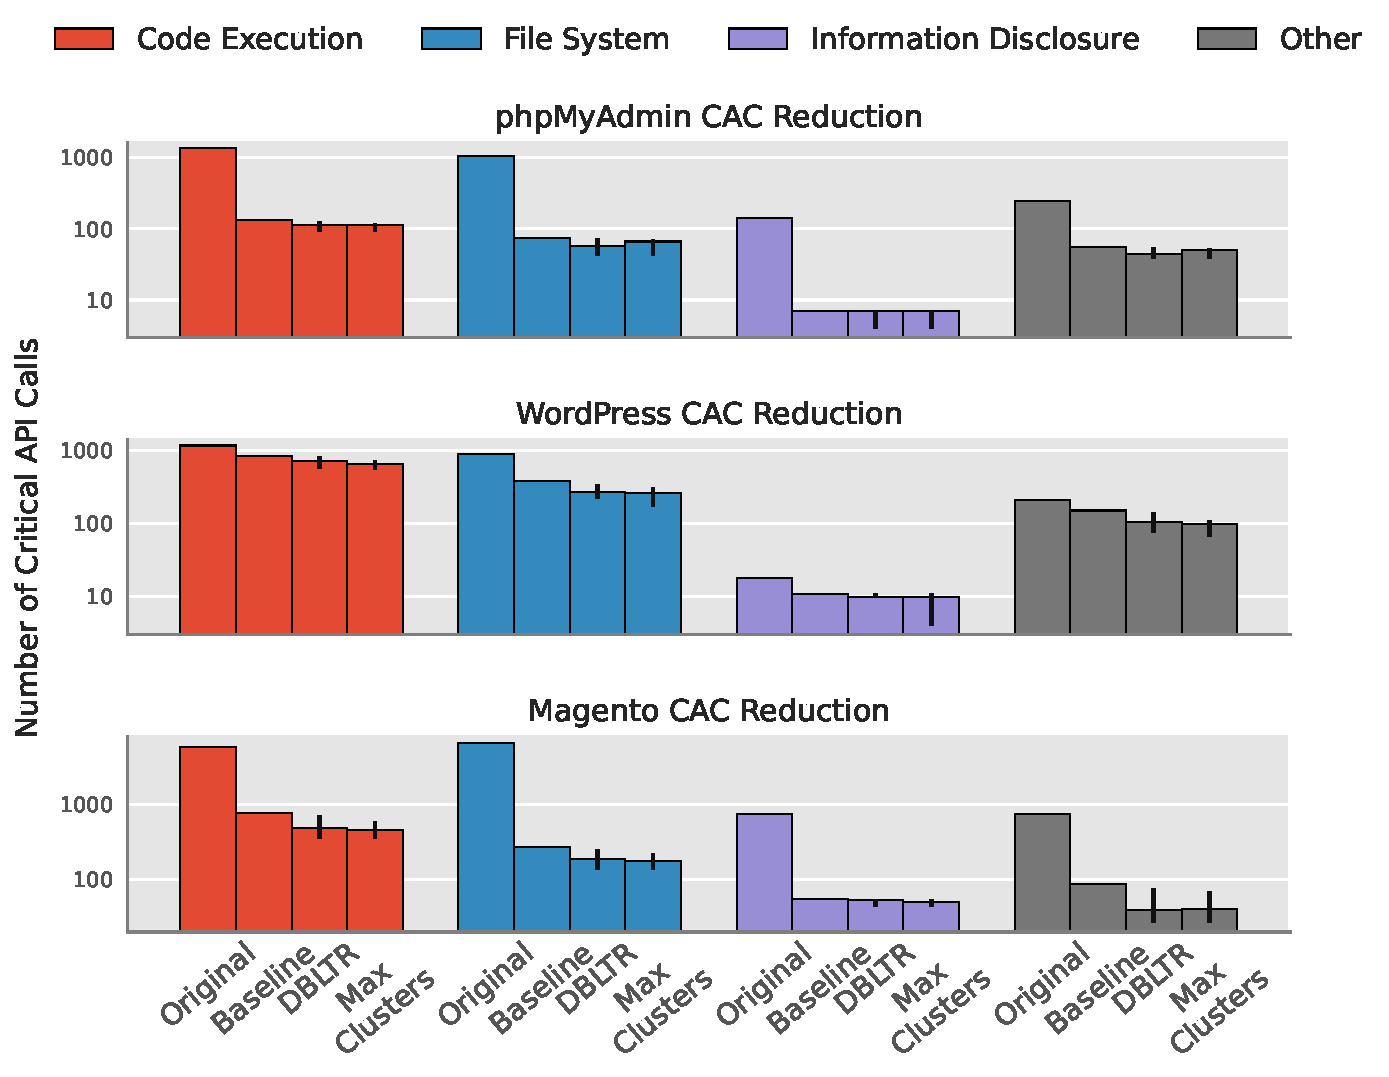
\includegraphics[width=0.65\textwidth]{figures/dbltr/cac_reduction.pdf}
    \caption{Critical API Call (CAC) reduction after debloating.}
    \label{fig:cac_reduction}
\end{figure}

Another security metric that we look at is the reduction in Critical API Calls (CACs). 
Figure~\ref{fig:cac_reduction} depicts the CAC reduction trend for various clusters. 
The first bar of each group shows the total number of CACs for the original web applications.
Next, the Baseline bar shows the cluster that includes all users grouped together to form a single cluster. 
Finally, the \sys{} bar refers to number of clusters optimally chosen via \sys{}'s Silhouette scores. whereas the Max Clusters bar refers to the extreme of placing each user in their own singleton cluster.
%Third bar is the Optimal-Cluster where \sys{} determines the number of clusters by maximizing the average Silhouette scores. 
%Finally, Max-Cluster denotes the scenario in which individual users receive their own custom debloated web applications. 

Across all CAC categories and all web applications, we observe a significant reduction for any method of debloating. 
This reduction indicates that the majority of CACs are in unused parts of the applications. Upon closer inspection of phpMyAdmin results, it becomes evident that 85\% of code execution APIs reside in the external dependencies of the web application. 
More importantly, debloating removed 99.98\% of these code execution APIs. 
This reduction clearly demonstrates the effect of third-party bloat where the majority of sensitive APIs are left unused by web application users. 

Contrasting the CAC reduction by the cluster size yields an interesting result. 
First, we observe that debloating has removed the majority of CACs from all clusters. 
For phpMyAdmin and Magento, \sys{} reduced the number of code execution APIs by 90\%. 
This essentially signifies that none of the users in our dataset ever interacted with the majority of these APIs. 
Similarly, for WordPress \sys{} removed  removed 27.5\% of all code execution APIs. 
For other categories of CACs, we observe a similar trend in reduction which ranges from 80-95\% for phpMyAdmin and Magento, and an average of 40\% reduction for WordPress CACs from File system, Information disclosure, and Other categories. 

\begin{table}[]
    \centering
    \caption{PHP Object Injection Gadgets statistics after debloating. Listing number of existing gadgets for Baseline and the ratio of clusters of \sys{} exposed to those gadgets.}
    \label{tab:poi_gadgets}
    \begin{tabular}{|l|l|c|c|c|}
    \hline
    \textbf{Web Application}          & \textbf{Package} & \textbf{Original} & \textbf{Baseline} & \textbf{\begin{tabular}[c]{@{}l@{}}\sys{}\end{tabular}} \\ \hline
    phpMyAdmin               & Guzzle  & 2        & 1         & 100\%              \\ \hline
    WordPress                & Generic & 1        & 0         & 0                \\ \hline
    \multirow{3}{*}{Magento} & Guzzle  & 3        & 2         & 83\%, 16\%       \\ \cline{2-5} 
                             & Magento & 1        & 1         & 16\%             \\ \cline{2-5} 
                             & Monolog & 6        & 0         & 0                \\ \hline
    \end{tabular}
\end{table}

The majority of CAC reduction occurs during the 1-Cluster baseline debloating. 
Nevertheless, smaller clusters can reduce CAC count by a further 10-40\% compared to the baseline, while the difference between \sys{} size and Max-cluster size is less than 5\% on average.
Therefore, from a CAC-reduction perspective, increasing the number of clusters past the Optimal-cluster size results in diminishing returns.

\subsubsection{PHP Object Injection Gadget Reduction}

\begin{table*}[]
    \centering
    \caption{Statistics on the contribution of cluster to individual code-coverage. 
    For files, third-party packages and first-party class modules, from the perspective of each individual user in the clusters, we show what percentage of those files or packages had new code-coverage by other users. Removed packages list the number of packages where a given percentage of their source code is removed by debloating.}
    \label{tab:augmented_coverage}
    \adjustbox{max width=\columnwidth}{
    \begin{tabular}{|l|c|c|c|c|c|ccc|}
    \hline
    \multirow{2}{*}{\textbf{Web Application}}   & \multirow{2}{*}{\textbf{\begin{tabular}[c]{@{}l@{}}\% Files with \\ new coverage\end{tabular}}} & \multirow{2}{*}{\textbf{\# Packages}} & \multirow{2}{*}{\textbf{\# Classes}} & \multicolumn{1}{c|}{\multirow{2}{*}{\textbf{Average Package}}} & \multirow{2}{*}{\textbf{Average Class}} & \multicolumn{3}{c|}{\textbf{Removed Packages}}                                                                       \\ \cline{7-9} 
                                                &                                                                                                 &                                       &                                      & \multicolumn{1}{c|}{}                                          &                                         & \multicolumn{1}{l|}{\textbf{\textgreater 70\%}} & \multicolumn{1}{l|}{\textbf{30\%-70\%}} & \textbf{\textless 30\%}  \\ \hline
    phpMyAdmin                                  & 18.5\%                                                                                          & 98                                    & 23                                   & 29\%                                                           & 72\%                                    & \multicolumn{1}{c|}{55}                         & \multicolumn{1}{c|}{18}                 & \multicolumn{1}{c|}{25}  \\ \hline
    WordPress                                   & 38.3\%                                                                                          & NA                                    & 23                                   & NA                                                             & 50\%                                    & \multicolumn{1}{c|}{NA}                         & \multicolumn{1}{c|}{NA}                 & \multicolumn{1}{c|}{NA}  \\ \hline
    Magento                                     & 15.3\%                                                                                          & 493                                   & 190                                  & 71\%                                                           & 68\%                                    & \multicolumn{1}{c|}{251}                        & \multicolumn{1}{c|}{164}                & \multicolumn{1}{c|}{78}  \\ \hline
    \end{tabular}
    }
\end{table*}

To identify existing object injection gadgets in the applications of our dataset, we incorporate PHPGGC~\cite{PHPGGC}, an open-source project listing available gadget chains for popular composer packages. 
After mapping the list of vulnerable package with those in phpMyAdmin, WordPress, and Magento, we search for the removal of classes and functions used within the gadget chains after debloating. 

Table~\ref{tab:poi_gadgets} lists the packages in each of our web applications with a known gadget chain based on PHPGGC. 
Under the column named ``Original'' we list the number of gadget chains within each package. 
As before, the Baseline column lists the number of gadget chains available after debloating, whereas the \sys{} column lists the percentage of the optimal number of clusters that contain those gadgets. 

The Guzzle package in phpMyAdmin includes 2 known gadget chains that can lead to arbitrary file write and code execution. 
Debloating the application into 1-Cluster (Baseline) removes one of these gadgets but the other gadget remains present across all clusters. 
For WordPress, the baseline debloating strategy removes the existing gadget therefore there are no opportunities for any additional gains by \sys{}.

More interestingly, Magento contains 10 known gadget chains. 
For Magento's Guzzle package, we observe that while 2 gadgets are still present in the Baseline debloating, (5/6) 83\% of clusters contain one gadget chain while only 16\% contain the other. 
For the gadget chain within the Magento package itself, only 16\% of clusters produced by the \sys{} contain this gadget. 

Our results confirm the findings of previous work that debloating is a highly effective defense for removing publicly known object injection gadget chains. 
Moreover, we observe that by clustering users into multiple groups, we can further breakdown the availability of gadgets and in certain cases, protect as much as 83\% of users and clusters against exploitation of an object injection vulnerability.

\subsection{Contribution of individual users to the overall code-coverage of clusters}
\label{sec:augmented_coverage}

Dynamic code-coverage data precisely models how users interact with web applications. 
One of the limitations of this modeling is that it overlooks the use cases that it has not seen before. 
As an example in our dataset, we observed that certain users executed queries that resulted only in a few rows. 
Therefore, some of the functions of the ``Display Results'' class of phpMyAdmin relating to pagination of results were never invoked. 
Meanwhile, other users with very similar usage behavior that ended up in the same cluster executed queries that exercised the pagination functions. 
As a result, all users within this cluster would retain this functionality and can run queries that result in a large number of rows.
In such scenarios, the clustering expands the available features for users with similar usage patterns. 

To quantify this effect, we look at the contribution of individual users in the cluster compared to the overall cluster code-coverage. 
For each user, we compare their file and function coverage information with all other users in the same cluster. 
To identify similar functionality that have been added to the cluster coverage by other users, we look at new lines covered in an already covered file. 
This modeling captures the effect of exercising new features within an already covered file.
Moreover, we investigate the inclusion of new files in the overall coverage within an existing module. 
For this purpose, we closely investigate the source code structure of the web applications in our dataset and identify the directory structure of their internal and external (e.g., composer) packages. 

\subsubsection{Analyzing module structures} By analyzing the code-base structure of the applications in our dataset, we made the following observations:

\textbf{phpMyAdmin} uses composer packages. As a result, external dependencies such as Twig, Symfony, Tcpdf, etc. are located under \texttt{vendor/package\_author/package\_name/} directory structure.
Similarly, phpMyAdmin stores internal modules and classes such as Charsets, Display, Export, etc. under \texttt{libraries/classes/module\_name/}. 
For phpMyAdmin, we identified 98 external and 23 internal modules.

\textbf{WordPress} unlike phpMyAdmin, does not use external composer packages. 
Nevertheless, WordPress modules are split into public and admin sections. 
Admin modules are located under \texttt{wp-admin/includes/class\_name} and public modules are under \texttt{wp-includes/class\_name}. 
Some examples of these modules are, PHPMailer, Requests, Rest-API, Widgets, etc.
Similarly, WordPress themes and plugins have their own unique directory under \texttt{wp-content/themes} and \texttt{wp-content/plugins} directory. 
For WordPress we identified 23 first-party modules. 

\textbf{Magento} incorporates multiple first-party and third-party modules via composer. 
Also, internal modules and classes are located under \texttt{app/code/Magento/module\_name} as well as \texttt{generated/code/module\_name}. 
From the Magento source code, we identified 493 external and 190 internal modules. 

Statistics on the code-coverage contribution of clusters to each individual user are available in Table~\ref{tab:augmented_coverage}. 
Under the column ``\% Files with new coverage'' we report the percentage of total files for which the cluster contributed new lines to the code-coverage of each individual member of that cluster. 
This number ranges from 15.3\% to 38.3\%, which signifies that a considerable number of functions for each class are included in the final code-coverage by other users in the same cluster. 

Table~\ref{tab:augmented_coverage} also lists the total number of third-party packages and first-party class modules. 
Clustering led to inclusion of new files for an average of 29\% to 71\% of packages, and 50\% to 72\% of class modules. 
On a similar note, these results quantitatively demonstrate that clustering users with similar behavior together leads to inclusion of similar functions, and therefore, reduces the likelihood of removing functions that are actually required by the users. 
Users who make extensive use of the necessary web-application features cluster together with users with more lightweight usage, allowing the latter to gradually expand their use without breaking the web application due to debloated code. 

Finally, we look at the number of ``Removed Packages'' for the clusters produced by \sys{} in Table~\ref{tab:augmented_coverage}. 
This column reports the number of packages in the web application where a given percentage of lines are removed after debloating.
These statistics show that for over half of the packages for phpMyAdmin and Magento, debloating has removed more than 70\% of their lines. 
In other words, while clustering users with similar behavior together expands their code-coverage of similar features significantly, the debloating procedure is still successfully removing the majority of the code from third-party dependencies, where majority of the bloated code resides~\cite{lessismore}.

\subsection{Performance of \sys}

We analyze the performance of \sys{} from two perspectives, request response time, and server resource utilization. 
Our test setup consists of an HTTP client and the web server. 
The HTTP clients simulate 100 users that send requests in parallel. 
Each client runs in a separate thread and sends batches of 40 requests (average number of requests to load the homepage of WordPress and its resources) towards the main page of WordPress hosted on a remote server. 
This setup simulates the work load for a website with 192,000 daily page views receiving 90 requests-per-second. 
We run each test for five minutes and repeat the tests five times and report the average statistics and remove the outliers. 

For the server setup, our web server hosts a WordPress website and we run each configuration in a containerized environment. 
We run our webservers on a server with 32GBs of RAM, and 32 Cores Intel Xeon E5-2440 CPUs running . 
We test the following setups:

\begin{itemize}
    \item \textbf{Single web server (Apache)} consists of one Apache webserver without a reverse-proxy. 
    \item \textbf{Baseline} is made up of an OpenResty reverse proxy and one Apache webserver. This setup serves as our baseline. 
    \item \textbf{\sys{} setups} expand the baseline setup by including the \sys{} modules and consist of one reverse-proxy and 1-50 Apache web servers. Each web server is responsible for the debloated web application for a specific role. This way, we measure the effect of the number of roles on the request response times. Under this setup, each client is assigned to one role in a round-robin fashion.
\end{itemize}

\begin{figure}[]
    \centering
    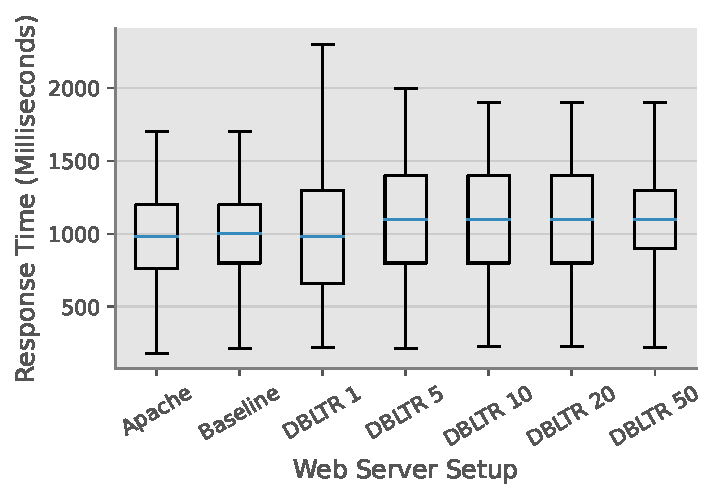
\includegraphics[width=0.55
    \textwidth]{figures/dbltr/performance.pdf}
    \caption{Distribution of request response time in milliseconds for Apache, Baseline, and \sys{} with a varying number of roles (i.e., backed Apache servers).}
    \label{fig:performance}
  \end{figure}

\subsubsection{Request Response Time Statistics}
We measure the request response time statistics from the perspective of our HTTP clients and report them in Figure~\ref{fig:performance}. 
The mere addition of the reverse-proxy (Baseline) increases the median response time of requests by 2\%. 
For \sys{}, the overhead from analysis and routing modules results in an average increase of 12\% in the median response time and 15\% increase in the 99th percentile response time. 
Moreover, a higher number of roles reduces the variance in the response times, as evident by the smaller boxes and shorter whiskers from one (DBLTR 1) to fifty roles (DBLTR 50). 

\subsubsection{Resource Utilization}
We measured the CPU and memory utilization of our test setup using the Docker runtime metrics API. 
Table~\ref{tab:performance} reports the resource usage statistics for the web servers and content-delivery (i.e., reverse-proxy) modules. 
Overall, the content-delivery module both in baseline and \sys{} setups utilizes 5-6\% of CPU and less than 20MiB of RAM which is very small compared to the amount of resources utilized by the web server. 
Moreover, across all setups, the CPU utilization of the web server modules remains constant. 
At the same time, increasing the number of roles in \sys{} which results in an increase in the number of web servers results in a linear increase in the overall memory utilization. 
During our tests, we observed a 5x increase in overall memory usage of \sys's web servers when increasing the number of roles by an order of 50x. 

\paragraph{Disk space utilization} \sys{} stores a separate and unique debloated copy of the web applications for each role. 
As a result, the disk utilization overhead of \sys{} is proportional to the number of roles. 
While shrinking the disk utilization of \sys{} is not a main goal, by definition, the debloating process removes unused lines of code. 
Overall, debloated web applications occupy 5-10\% less disk space. 
While this reduction may be insignificant for smaller web applications, for larger ones such as Magento, debloated web applications on average occupy 100MB less disk space. 


\begin{table}[]
    \centering
    \caption{Average CPU and Memory utilization of \sys. \textit{DBLTR N}-Web Servers row shows the range of CPU and Memory utilization for \textit{DBLTR 1} to \textit{DBLTR 50}.}
    \label{tab:performance}
    \adjustbox{max width=\columnwidth}{
    \begin{tabular}{|l|l|l|l|}
    \hline
    \textbf{Setup}                    & \textbf{Module}  & \textbf{Avg CPU} & \textbf{Avg Memory (MiB)} \\ \hline
    Apache                            & Web Server       & 3117\%              & 2378                            \\ \hline
    \multirow{2}{*}{Baseline}         & Content-Delivery & 6\%                 & 17                           \\ \cline{2-4} 
                                      & Web Server       & 3057\%              & 2332                         \\ \hline
    \multirow{2}{*}{\textit{DBLTR N}} & Content-Delivery & 6\%                 & 19                           \\ \cline{2-4} 
                                      & Web Servers      & 2905-3072\%      & 2179-10374                \\ \hline
    \end{tabular}
    }
\end{table}